
\begin{frame}{Đặt vấn đề}
    \begin{itemize}
        \item \textbf{Thực trạng:} Ảnh giám sát giao thông thường bị suy giảm chất lượng do:
        \begin{itemize}
            \item Điều kiện ánh sáng kém, thời tiết xấu gây nhiễu
            \item Chuyển động nhanh gây mờ 
            \item Giới hạn phần cứng thiết bị ghi/xử lý hình ảnh
        \end{itemize}
        \item \textbf{Hậu quả:}
        \begin{itemize}
            \item Giảm độ chính xác của hệ thống nhận diện biển số (ANPR/OCR)
            \item Sai lệch trong xử lý vi phạm và quản lý giao thông
            \item Ảnh hưởng đến điều tra an ninh
        \end{itemize}
        \item \textbf{Thách thức:}
        \begin{itemize}
            \item Cần bảo toàn chi tiết ảnh để không ảnh hưởng các thao tác nhận diện biển số
            \item Yêu cầu xử lý thời gian thực trên thiết bị nhúng
        \end{itemize}
        \item \textbf{Giải pháp:}
        \begin{itemize}
            \item Kiến trúc cải tiến của mã hóa tự động có bổ sung thiết kế phụ trợ để cải tiến khả năng khôi phục ảnh và tối ưu tham số mô hình 
        \end{itemize}
    \end{itemize}
\end{frame}

\begin{frame}{Bài báo tại hội nghị SOICT 2025}
    \begin{columns}
        \begin{column}{0.5\textwidth}
            \begin{figure}
                \centering
                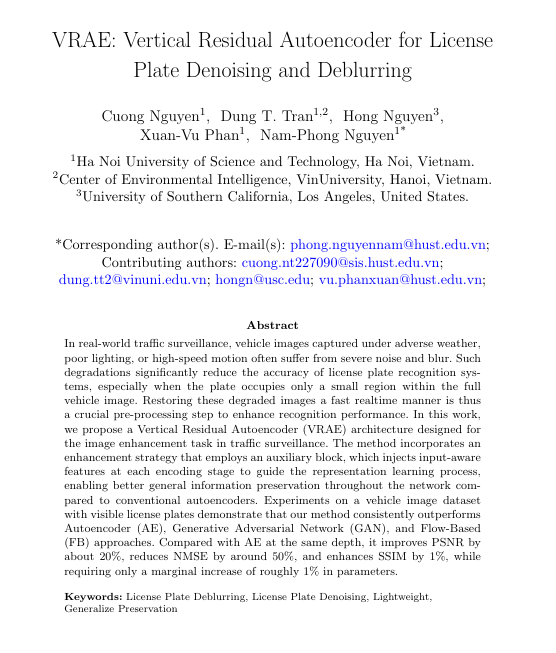
\includegraphics[width=\linewidth]{images/first_page_paper.png}
                % \caption{Thay đổi Entropy }
            \end{figure}
        \end{column}
        \begin{column}{0.4\textwidth}
            \textbf{Hội nghị SOICT 2025}
            \begin{itemize}
                \item Hội nghị quốc tế lần thứ 14 về công nghệ thông tin và truyền thông
                \item Năm 2025, SOICT thu hút hơn 327 bài gửi từ 30 quốc gia.
                \item Lĩnh vực: Khoa học máy tính, trí tuệ nhân tạo, khoa học dữ liệu, thông tin và truyền thông, v.v.
            \end{itemize}
        \end{column}
    \end{columns}
\end{frame}

% \subsection{Mục tiêu nghiên cứu}
% \begin{frame}{Mục tiêu nghiên cứu}
%     \small
%     \begin{enumerate}
%         \item Đề xuất phương pháp khử nhiễu và khử mờ hiệu quả cho ảnh phương tiện, tập trung vào việc bảo toàn chi tiết vùng biển số
%         \item Tối ưu hóa mô hình về số tham số và chi phí tính toán để phù hợp triển khai trên thiết bị thực tế
%         \item Đánh giá hiệu quả bằng các chỉ số ảnh kỹ thuật (PSNR, SSIM) và tỷ lệ nhận diện biển số sau xử lý
%     \end{enumerate}
    
%     \vspace{0.1cm}
%     \textbf{Đo lường hiệu quả:}
%     \begin{itemize}
%         \item PSNR (Peak Signal-to-Noise Ratio)
%         \item SSIM (Structural Similarity Index)
%         \item NMSE (Normalized Mean Squared Error)
%         \item Thời gian xử lý và kích thước mô hình
%     \end{itemize}
% \end{frame}
